% geodesic_math.tex: the formulas of Dubins_TSP_New_Implementation_claude/geodesic.py,
% in the notation and style of Section 0.13 of Dubins_TSP.pdf.
%
% Build from this folder (needs the figures from make_figures.py):
%   python make_figures.py
%   python check_formulas.py      # the checks of the section "How the Statements Were Checked" (about 3 minutes)
%   pdflatex geodesic_math.tex && pdflatex geodesic_math.tex
%   mv geodesic_math.pdf ..
\documentclass[10pt]{article}
\usepackage[letterpaper,margin=1in]{geometry}
\usepackage{amsmath,amssymb}
\usepackage{graphicx}
\usepackage{booktabs}
\usepackage{array}
\usepackage{tabularx}
\usepackage{enumitem}
\usepackage{float}
\usepackage[font=small,labelfont=bf]{caption}
\usepackage[hidelinks]{hyperref}

\newcommand{\code}[1]{\texttt{#1}}
\newcommand{\rplan}{r_{\mathrm{plan}}}
\newcommand{\rsafe}{r_{\mathrm{safe}}}
\newcommand{\rterm}{r_{\mathrm{term}}}
\newcommand{\dgeo}{d_{\mathrm{geo}}}
\newcommand{\pred}{\mathrm{pred}}
\newcommand{\R}{\mathbb{R}}
\makeatletter\@secpenalty=0\makeatother   % do not prefer page breaks before headings

\begin{document}

\begin{center}
  {\LARGE Geodesic Distances: the Mathematics of \code{geodesic.py}}\\[1.2em]
  {\large November 2026}
\end{center}
\vspace{1em}

{\sloppy
This note explains how \code{geodesic.py} (in \code{Dubins\_TSP\_New\_Implementation\_claude/}) computes the
obstacle-aware distances of the paper: $r_i$ of eq.~(9), the matrix $D_{\mathrm{geo}}$ of Step~1 of Section~0.9, and
the obstacle-free paths that Step~2 of Section~0.11 builds on. It states every formula the code uses, in the notation of
\code{Dubins\_TSP.pdf}. Section~\ref{sec:idea} gives the idea in a few lines. Sections~\ref{sec:inflate}--\ref{sec:dijkstra}
give the formulas step by step, Section~\ref{sec:meaning} says what the result is and is not, and
Section~\ref{sec:checks} says how each statement was checked. Table~\ref{tab:notation}, in the appendix, lists every
symbol with its name in the code.\par}

\section{The Idea in Brief}
\label{sec:idea}

A sink cannot drive through an obstacle, so when an obstacle is in the way the straight-line distance between two
points is too short. The \emph{geodesic distance} is the length of the shortest path that goes round the obstacles.
\code{geodesic.py} finds it in four steps (Figure~\ref{fig:graph}):
\begin{enumerate}[leftmargin=2em, itemsep=2pt]
  \item \textbf{Grow the obstacles} (\code{inflate}). Each obstacle is enlarged by a safety margin, so a path that stays
        outside the grown obstacle keeps about that distance from the real one.
  \item \textbf{Decide which straight lines are allowed} (\code{\_inside}). A straight line is allowed if it does not cut
        into a grown obstacle. Touching it, or running along its edge, is allowed.
  \item \textbf{Build a graph} (\code{build}). Its \emph{nodes} are the base, the sensors and the corners of the grown
        obstacles. Two nodes are joined by an \emph{edge} if the straight line between them is allowed, and the edge's
        length is its \emph{weight}.
  \item \textbf{Find shortest paths} (\code{build}, \code{path}). Dijkstra's algorithm [2] finds the shortest chain of
        edges from each terminal (the base or a sensor) to every other terminal. Its length is the geodesic distance, and the chain
        itself is the obstacle-free path.
\end{enumerate}
Why corners are enough: a shortest path round polygons is like a string pulled tight. It consists of straight pieces
that bend only at corners of the obstacles [1, 3]. So the graph contains the shortest path, and no other bending points
are needed.

One detail differs from the textbook method: the code uses two margins. A line between two corners must stay outside the
obstacles grown by 7\,m, but a line that touches the base or a sensor only outside those grown by 2.5\,m (Section~2).

\begin{figure}[t]
  \centering
  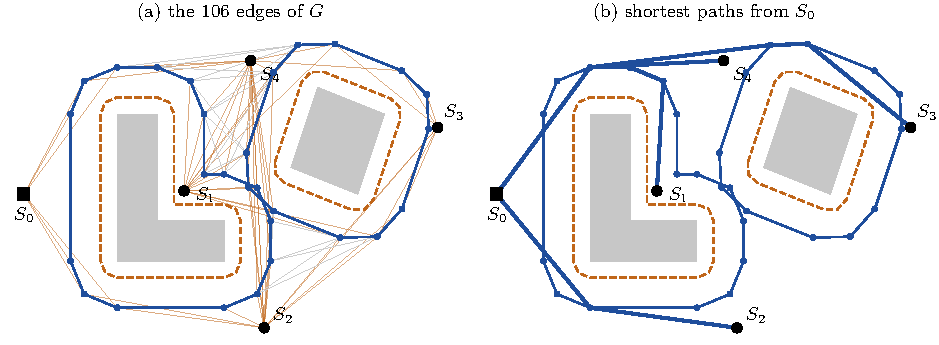
\includegraphics[width=\textwidth]{fig_graph.pdf}
  \caption{A small example, computed by \code{geodesic.build}: two obstacles (grey), the base $S_0$ (square) and four
  sensors. The blue polygons are the obstacles grown by $\rplan = 7$\,m; their 28 corners (blue dots) are graph nodes.
  The dashed orange polygons are the obstacles grown by $\rterm = 2.5$\,m. (a) Of the 528 pairs of nodes, 106 are joined:
  61 lines that touch the base or a sensor, allowed because they stay out of the orange polygons (orange), and 45 lines
  between two corners, allowed because they stay out of the blue polygons (grey). (b) The shortest path from $S_0$ to
  each sensor. $S_1$ sits in the inside corner of the L, within the blue polygon, so only a line tested against the orange
  polygon can reach it.}
  \label{fig:graph}
\end{figure}

\section{Obstacles, Sensors and Margins}

The field contains $m$ polygonal obstacles $O_1, \ldots, O_m$, the base station $S_0 = (x_0, y_0)$ and the sensors
$S_i = (x_i, y_i)$, $i = 1, \ldots, n$. The base and the sensors together are called the $n_t = n + 1$
\emph{terminals}, numbered $0, 1, \ldots, n$ as in the paper. In the code, terminal 0 is the base and terminal $i$ is
\code{scen["xy"][i - 1]}, the sensor with the 0-based id $i - 1$.

The paper defines the free space by growing the obstacles by a safety clearance, eqs.~(4) and~(5):
\begin{equation}
  F = \R^2 \setminus \bigcup_{j=1}^{m} \operatorname{int}\bigl(O_j^{\mathrm{inflated}}\bigr), \qquad
  \rsafe = \frac{w}{2} + \delta_{\mathrm{margin}}.
  \label{eq:free}
\end{equation}
\code{geodesic.py} uses two larger margins built on $\rsafe$:
\begin{equation}
  \rsafe = 2\,\mathrm{m}, \qquad
  \rterm = \rsafe + 0.5\,\mathrm{m} = 2.5\,\mathrm{m}, \qquad
  \rplan = \rsafe + R = 7\,\mathrm{m},
  \label{eq:margins}
\end{equation}
with the turning radius $R = L / \tan\delta_{\max} = 5$\,m of eq.~(7) and the defaults of \code{config.py}.
\begin{itemize}[leftmargin=2em, itemsep=2pt]
  \item $\rplan$ applies to lines between two obstacle corners. The extra $R$ leaves the sink room to turn where the path
        bends at a corner.
  \item $\rterm$ applies to lines that start or end at a terminal. Sensors may lie closer to an obstacle than $\rplan$ (on
        seeds 1--10, 577 of the 1\,015 sensors do), and they could never be reached if every line to them needed 7\,m.
        The code has no name for $\rterm$; it writes \code{p["r\_safe"] + 0.5}.
  \item $\rsafe$ itself is not used in \code{geodesic.py}. The clearance of the final trajectory is checked against it
        later (Section~\ref{sec:meaning}).
\end{itemize}
Table~\ref{tab:constants} lists every constant of the file.

\begin{table}[h]
\centering
\small
\caption{Constants in \code{geodesic.py}, with the defaults of \code{config.py}.}
\label{tab:constants}
\begin{tabularx}{\textwidth}{@{}l l >{\raggedright\arraybackslash}X@{}}
\toprule
Constant & Value & Role \\
\midrule
$\rplan = \rsafe + R$ & 7\,m & growth for the corner nodes and for lines between two corners \\
$\rterm = \rsafe + 0.5$ & 2.5\,m & growth for lines that start or end at a terminal \\
$q$ (\code{quad\_segs}) & 2 & sets the chord size at the corners of a grown obstacle, eq.~\eqref{eq:nchords} \\
$\varepsilon$ & $10^{-6}$\,m & how far a line may enter a grown obstacle, eq.~\eqref{eq:inside} \\
\code{require\_all} & \code{True} & stop if a terminal cannot be reached (\code{scenario.py} passes \code{False}) \\
\bottomrule
\end{tabularx}
\end{table}

\section{Step 1: Growing the Obstacles}
\label{sec:inflate}

\emph{In words:} \code{inflate} replaces each obstacle by a polygon that is larger by about $r$ all round.

The exact grown obstacle is the set of points within $r$ of the obstacle:
\begin{equation}
  G_r(O_k) = \bigl\{ x \in \R^2 : \operatorname{dist}(x, O_k) \le r \bigr\}.
  \label{eq:grown}
\end{equation}
Its corners are round. The code uses a polygon $P_r(O_k)$ in its place, made by shapely's \code{buffer} with
\code{quad\_segs} $= q = 2$. Its boundary follows four rules (Figure~\ref{fig:inflate}).

\begin{figure}[t]
  \centering
  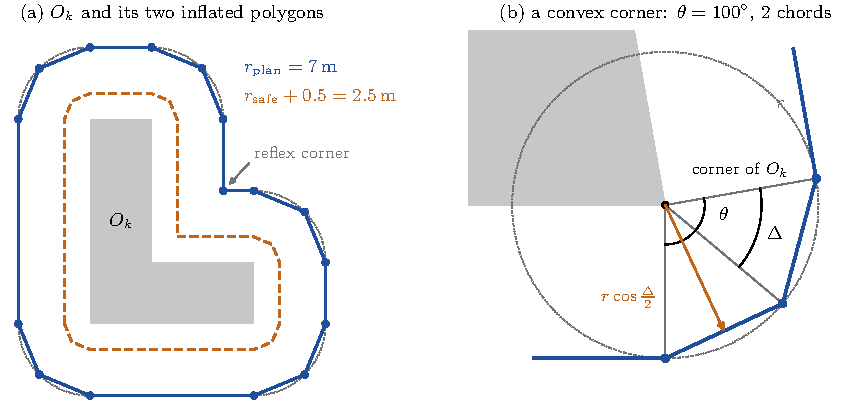
\includegraphics[width=\textwidth]{fig_inflate.pdf}
  \caption{(a) An L-shaped obstacle (16\,m by 20\,m, arms 6\,m wide) grown by 7\,m (blue; its 12 corners become graph
  nodes) and by 2.5\,m (dashed orange), as \code{geodesic.inflate} makes them. The dotted line is the exact grown
  obstacle of eq.~\eqref{eq:grown}, with round corners. At the inside corner of the L the two moved edges simply meet.
  (b) One outer corner, where the boundary turns through $\theta = 100^\circ$. Eq.~\eqref{eq:nchords} gives 2 chords of
  $\Delta = 50^\circ$. Their ends lie on the circle of radius $r$, and their midpoints are $r\cos 25^\circ = 0.906\,r$ from
  the corner.}
  \label{fig:inflate}
\end{figure}

\paragraph{1. Edges.} Each edge of $O_k$ is moved outward, parallel to itself, by $r$.

\paragraph{2. Outer (convex) corners.} Here the round arc of $G_r$ is replaced by straight chords. Let $\theta$, between
$0$ and $\pi$, be the angle through which the boundary turns at the corner $c$: the angle between the outward normals of
the edge arriving at $c$ and the edge leaving it. The arc is cut into
\begin{equation}
  n_\theta = \max\Bigl(1,\ \Bigl\lfloor \frac{4\theta}{\pi} + \frac{1}{2} \Bigr\rfloor\Bigr)
  \quad\text{equal chords, each turning through}\quad \Delta = \frac{\theta}{n_\theta}.
  \label{eq:nchords}
\end{equation}
In words: the arc is cut into pieces of about $45^\circ$ (that is, $\pi/(2q)$ with $q = 2$), with the number rounded to the
nearest whole number but at least one. A right-angled corner gets two chords of $45^\circ$. The chord ends lie on the
circle of radius $r$ about the corner:
\begin{equation}
  c + r\,\bigl(\cos(\varphi_0 + j\Delta),\ \sin(\varphi_0 + j\Delta)\bigr), \qquad j = 0, 1, \ldots, n_\theta,
  \label{eq:fillet}
\end{equation}
where $\varphi_0$ is the direction of the outward normal of the arriving edge, and the angle grows in the direction in which
the boundary turns.

\paragraph{3. Inner (reflex) corners.} At a corner such as the inside corner of an L, the two moved edges cross, and
the crossing point is the corner of the polygon.

\paragraph{4. Overlaps.} Where the moved boundary overlaps itself, as in the pocket of a C or the notches of a cross, the
polygon is the union of the pieces, so the covered parts of the boundary disappear.

\paragraph{How close the polygon comes to the obstacle.} A chord lies inside the circle, so it comes closer to the
corner than $r$: its midpoint is $r\cos(\Delta/2)$ away. The worst case is the largest $\Delta$. By
eq.~\eqref{eq:nchords}, a corner gets a single chord only if $\theta < 67.5^\circ$, and $n \ge 2$ chords only if
$\theta < (n + \frac{1}{2}) \cdot 45^\circ$, so
\begin{equation}
  \Delta < 67.5^\circ = \frac{3\pi}{8}, \qquad
  r\cos\frac{\Delta}{2} > r\cos\frac{3\pi}{16} = 0.8315\,r.
  \label{eq:sag}
\end{equation}
No vertex is farther than $r$ from the obstacle. Together with eq.~\eqref{eq:sag}, every point $x$ on the boundary of
the polygon satisfies
\begin{equation}
  \boxed{0.8315\,r \ \le\ \operatorname{dist}(x, O_k) \ \le\ r.}
  \label{eq:inclusion}
\end{equation}
Equivalently, $P_r(O_k)$ contains $G_{0.8315\,r}(O_k)$ and lies inside $G_r(O_k)$. So the polygon grown by
$\rterm = 2.5$\,m keeps at least 2.08\,m from the obstacle, more than $\rsafe = 2$\,m; the polygon grown by
$\rplan = 7$\,m keeps at least 5.82\,m; and since $5.82 > 2.5$, the 2.5\,m polygon lies inside the 7\,m polygon.

\section{Step 2: Which Straight Lines Are Allowed}

\emph{In words:} a line is allowed if it does not cut into a grown obstacle; a tiny tolerance lets it touch.

The function \code{\_inside} takes the inside of the grown obstacles, shrunk by $\varepsilon = 10^{-6}$\,m:
\begin{equation}
  I_r = \bigl\{ x : \text{for some } k,\ x \text{ and every point within } \varepsilon \text{ of it lie in } P_r(O_k) \bigr\}.
  \label{eq:inside}
\end{equation}
A straight line from $p$ to $q$ is \emph{allowed at margin $r$} if it has no point in $I_r$:
\begin{equation}
  [p, q] \cap I_r = \emptyset.
  \label{eq:clear}
\end{equation}
Why shrink: shapely counts touching as meeting. Without the shrinking, a line running along the edge of a grown obstacle
would be refused, and so would every line from a corner node, because the corner lies on the edge. With it, a line may
touch the polygon, run along its edge, or enter it by at most $\varepsilon$. By eq.~\eqref{eq:inclusion}, an allowed line
keeps at least $0.8315\,r - \varepsilon$ from every obstacle.

\section{Step 3: The Graph}

\emph{In words:} the nodes are the terminals and the corners of the 7\,m polygons; two nodes are joined if the line
between them is allowed at the margin that applies to it.

\paragraph{Nodes} (\code{build}). The terminals come first, then the corners:
\begin{equation}
  \begin{aligned}
  &v_a = S_a \quad (a = 0, \ldots, n),\\
  &v_{n_t}, \ldots, v_{N-1} = \text{the vertices of the outer boundaries of } P_{\rplan}(O_1), \ldots, P_{\rplan}(O_m).
  \end{aligned}
  \label{eq:nodes}
\end{equation}
If a polygon had a hole, the corners of the hole would not be nodes.

\paragraph{Edges.} Every pair of nodes $a < b$ is tested once. Because the terminals come first, the line touches a
terminal exactly when $a < n_t$:
\begin{equation}
  \boxed{\text{$a$ and $b$ are joined} \iff
  \begin{cases}
    [v_a, v_b] \cap I_{\rterm} = \emptyset & \text{if } a < n_t \text{ (the line starts or ends at a terminal)},\\
    [v_a, v_b] \cap I_{\rplan} = \emptyset & \text{if } a \ge n_t \text{ (the line joins two corners)}.
  \end{cases}}
  \label{eq:edges}
\end{equation}
If there are no obstacles, every pair is joined. The weight of an edge is its length,
\begin{equation}
  w_{ab} = \lVert v_a - v_b \rVert = \sqrt{(x_a - x_b)^2 + (y_a - y_b)^2},
  \label{eq:weight}
\end{equation}
and the graph is undirected: the edge can be used both ways. With $N$ nodes, $N(N - 1)/2$ pairs are tested. On seed~1
there are 99 terminals and 148 corner nodes: 30\,381 pairs, of which 7\,898 are joined (6\,800 touching a terminal and
1\,098 between two corners).

\section{Step 4: Shortest Distances and Paths}
\label{sec:dijkstra}

\emph{In words:} the geodesic distance is the length of the shortest chain of edges, and Dijkstra's algorithm finds it.

\paragraph{Geodesic distance.} For terminals $a$ and $b$,
\begin{equation}
  \boxed{D_{ab} = \min\Bigl\{ \sum_{l=1}^{L} w_{u_{l-1} u_l} \ :\ u_0 = a,\ u_L = b,\
  \text{each } u_{l-1}, u_l \text{ joined} \Bigr\},}
  \label{eq:D}
\end{equation}
the smallest total length of a chain of edges $a = u_0, u_1, \ldots, u_L = b$. If no chain exists, $D_{ab} = \infty$.

\paragraph{Dijkstra's algorithm} (\code{dijkstra}), run once from each terminal $a = 0, \ldots, n$. It spreads out from
$a$ in order of distance, like a wave. It starts with $d_a(a) = 0$ and $d_a(v) = \infty$ for every other node. Then, again
and again, it fixes the nearest node $u$ not yet fixed, and checks whether going through $u$ shortens the path to each
neighbour $v$:
\begin{equation}
  \text{if } d_a(u) + w_{uv} < d_a(v): \qquad d_a(v) \leftarrow d_a(u) + w_{uv}, \qquad \pred_a(v) \leftarrow u.
  \label{eq:relax}
\end{equation}
$\pred_a(v)$ remembers the node before $v$ on the best path found so far. When the algorithm stops, each reachable node's
distance is the best ``distance of a neighbour plus the last edge'':
\begin{equation}
  d_a(v) = \min_{u \text{ joined to } v} \bigl( d_a(u) + w_{uv} \bigr) \quad (v \ne a),
  \label{eq:bellman}
\end{equation}
and $D_{ab} = d_a(b)$. The code keeps $D = (D_{ab})$, an $n_t \times n_t$ matrix over the terminals.

\paragraph{The paper's distances.} Eq.~(9) and Step~1 of Section~0.9 are entries of $D$:
\begin{equation}
  r_i = \dgeo(S_0, S_i) = D_{0i}, \qquad
  D_{\mathrm{geo}} = \bigl[\dgeo(i, j)\bigr] = \bigl[D_{ij}\bigr]_{i, j = 1, \ldots, n}.
  \label{eq:paper}
\end{equation}
In the code these are \code{geo["D"][0, 1:]} and \code{geo["D"][1:, 1:]}, with 0-based sensor ids. In
Figure~\ref{fig:graph}, $S_1$ is 24.0\,m from the base in a straight line, but the L is in the way, and the path over the
top of the L gives $D_{01} = 51.4$\,m. For the other sensors $D_{0i}$ is 44.2, 76.2 and 43.6\,m, against straight-line
distances of 41.2, 62.8 and 39.5\,m.

\paragraph{The path} (\code{path}). Follow the predecessors back from $b$ until $a$ is reached, then read the nodes
forward:
\begin{equation}
  u_L = b, \qquad u_{l-1} = \pred_a(u_l) \ \text{ until } u_0 = a, \qquad
  \Gamma_{ab} = \bigl( v_{u_0}, v_{u_1}, \ldots, v_{u_L} \bigr).
  \label{eq:path}
\end{equation}
$\Gamma_{ab}$ is a chain of straight lines from $S_a$ to $S_b$ of length $D_{ab}$, defined only when $D_{ab} < \infty$.
\code{trajectory.py} uses its nodes as the waypoints of a leg.

\paragraph{Unreachable terminals.} If some $D_{ab} = \infty$, \code{build} stops with the error ``some sensors cannot be
reached from the base station''. \code{scenario.py} calls it with \code{require\_all=False} instead, to drop candidate
sensors that cannot be reached.

\section{What \texorpdfstring{$D$}{D} Is, and What It Is Not}
\label{sec:meaning}

\begin{figure}[t]
  \centering
  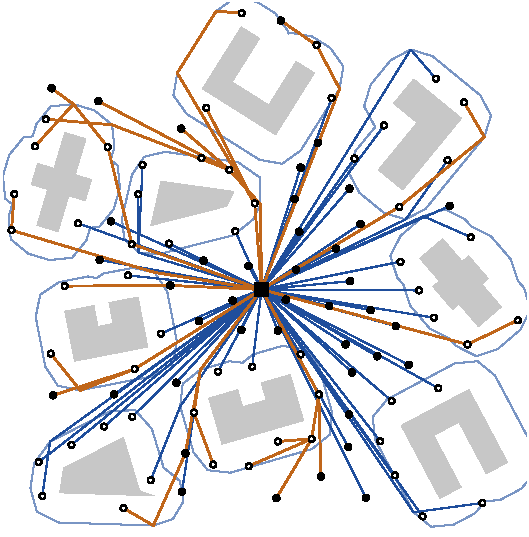
\includegraphics[width=0.52\textwidth]{fig_seed1.pdf}
  \caption{Seed 1 with the default settings: 9 obstacles (grey), the obstacles grown by 7\,m (thin blue outline), the
  base (square) and 98 sensors. The 57 hollow sensors lie inside the 7\,m outline. The lines are the shortest paths
  $\Gamma_{0i}$ from the base. The 23 orange paths pass through another sensor and bend there with only the 2.5\,m margin;
  the blue ones bend only at corners of the 7\,m polygons. Some paths go round obstacles that reach beyond the 100\,m map.}
  \label{fig:seed1}
\end{figure}

\paragraph{It behaves like a distance.} Because $D$ is a shortest-path length in an undirected graph with lengths as
weights,
\begin{equation}
  D_{aa} = 0, \qquad D_{ab} = D_{ba}, \qquad D_{ac} \le D_{ab} + D_{bc}, \qquad D_{ab} \ge \lVert S_a - S_b \rVert.
  \label{eq:metric}
\end{equation}
That is: zero from a point to itself, the same both ways, never longer than going via a third terminal, and never shorter
than the straight line.

\paragraph{It lies between the true distances at the two margins.} If every line were tested at one margin, $D$ would be
the exact length of the shortest path round the obstacles grown by that margin, because such a path bends only at corners
[1, 3]. With two margins, $D$ lies between the two exact lengths. Write $d(p, q; X)$ for the length of the shortest path
from $p$ to $q$ that has no point in the set $X$. Then
\begin{equation}
  \boxed{d\bigl(S_a, S_b;\ I_{\rterm}\bigr) \ \le\ D_{ab} \ \le\
  d\Bigl(S_a, S_b;\ \operatorname{int} \textstyle\bigcup_k P_{\rplan}(O_k)\Bigr),}
  \label{eq:bounds}
\end{equation}
where the right-hand side needs $S_a$ and $S_b$ to lie outside the 7\,m polygons. In words: $D$ is never shorter than the
shortest path that stays out of the 2.5\,m polygons, and never longer than the shortest path that stays out of the 7\,m
polygons. The lower bound holds because every edge is allowed at 2.5\,m; a line allowed at 7\,m is also allowed at 2.5\,m,
since the 2.5\,m polygon lies inside the 7\,m one. The upper bound holds because the shortest path that stays out of the
7\,m polygons bends only at their corners, which are nodes, and each of its lines passes the test of
eq.~\eqref{eq:edges}.

\paragraph{Paths can pass through other sensors.} The terminals are nodes too, so a chain in eq.~\eqref{eq:D} may pass
through another sensor. Both of its lines at that sensor are tested only at 2.5\,m, so a sensor close to an obstacle can
act as a tighter corner than the corners of the 7\,m polygons (Figure~\ref{fig:seed1}). On seeds 1--10, 245 of the
1\,015 shortest paths from the base pass through another terminal.

\paragraph{What is not guaranteed here.} $D$ and $\Gamma_{ab}$ describe chains of straight lines, not the Dubins paths the
sinks drive. An allowed line keeps $0.8315\,\rterm - \varepsilon \ge 2.08$\,m from the obstacles if it touches a
terminal, and $0.8315\,\rplan - \varepsilon \ge 5.82$\,m if it joins two corners. But a Dubins path that follows the
waypoints can swing wider or cut inside. So eq.~(19) of the paper is checked on the final trajectory $\Gamma_k$ instead,
against the original obstacles, whose union \code{build} also returns:
\begin{equation}
  O = \bigcup_{k=1}^{m} O_k, \qquad \operatorname{dist}\bigl(\Gamma_k(t), O\bigr) \ge \rsafe .
  \label{eq:clearance}
\end{equation}

\section{How the Statements Were Checked}
\label{sec:checks}

\code{check\_formulas.py}, next to the source of this note, repeats every check below.
\begin{itemize}[leftmargin=2em, itemsep=2pt]
  \item \textbf{Chords at the corners}, eqs.~\eqref{eq:nchords}--\eqref{eq:inclusion}. 3\,000 random obstacles made by
        \code{scenario.py} (random polygons, L, C and cross shapes) were grown by 2.5\,m and by 7\,m. All 29\,047 outer
        corners whose arc lies on the boundary have exactly the vertices of eq.~\eqref{eq:fillet}. At the other 6\,119,
        another arm of the same obstacle covers part of the arc (rule 4). The largest chord angle was $67.44^\circ$, the
        closest approach of a boundary to its obstacle $0.8318\,r$, and the farthest vertex lay at $r$ to within
        $10^{-11}r$.
  \item \textbf{Holes.} None of the 108 polygons grown by 7\,m on seeds 1--10 has a hole, so no corner is left out of
        eq.~\eqref{eq:nodes}.
  \item \textbf{Distance properties}, eq.~\eqref{eq:metric}. On seeds 1--10, $D$ was symmetric and met the triangle
        inequality to within $6 \times 10^{-14}$\,m, and never fell below the straight-line distance.
  \item \textbf{Bounds}, eq.~\eqref{eq:bounds}. On seeds 1--10, both bounds held for every pair of terminals, with the
        exact distances computed by visibility graphs tested at one margin only.
  \item \textbf{Counts.} On seeds 1--10, 577 of 1\,015 sensors lie inside the 7\,m polygons, and 245 of the 1\,015 paths
        from the base pass through another terminal.
\end{itemize}

\section{Relation to the Paper}

The paper says what $\dgeo$ is (eq.~(9): ``an obstacle-aware geodesic walking distance in the free space''; Step~1 of
Section~0.9: ``the shortest obstacle-respecting distance''; and ``visibility-based'' geometry in the introduction of
Section~0.9), but not how to compute it. The code fills the gaps as in Table~\ref{tab:paper}; the README of the
implementation records the same choices in its table ``Choices where the paper is silent''.

\begin{table}[h]
\centering
\small
\caption{The paper and \code{geodesic.py}.}
\label{tab:paper}
\begin{tabularx}{\textwidth}{@{}>{\raggedright}p{0.22\textwidth} >{\raggedright}p{0.3\textwidth} >{\raggedright\arraybackslash}X@{}}
\toprule
Topic & Paper & \code{geodesic.py} \\
\midrule
Margin & $\rsafe$, eqs.~(4)--(5) & $\rplan$ and $\rterm$ in the graph, eq.~\eqref{eq:edges}; $\rsafe$ on the final path, eq.~\eqref{eq:clearance} \\
Shape of a grown obstacle & not given & polygon with chords at the corners, eqs.~\eqref{eq:nchords}--\eqref{eq:inclusion} \\
How $\dgeo$ is computed & ``visibility-based'' & visibility graph and Dijkstra, eqs.~\eqref{eq:nodes}--\eqref{eq:D} \\
Sensors near obstacles & not covered & lines that touch a terminal use $\rterm$, eq.~\eqref{eq:edges} \\
Paths via sensors & not covered & allowed, eq.~\eqref{eq:D} \\
Unreachable sensors & not covered & an error, or dropped by \code{scenario.py} \\
\bottomrule
\end{tabularx}
\end{table}

\section*{References}

[1] T. Lozano-P\'erez and M. A. Wesley, ``An algorithm for planning collision-free paths among polyhedral obstacles,''
Communications of the ACM, vol.~22, no.~10, pp.~560--570, 1979.

[2] E. W. Dijkstra, ``A note on two problems in connexion with graphs,'' Numerische Mathematik, vol.~1, pp.~269--271,
1959.

[3] M. de Berg, O. Cheong, M. van Kreveld and M. Overmars, Computational Geometry: Algorithms and Applications, 3rd ed.,
Springer, 2008, Chapter~15 (Visibility Graphs).

\appendix
\section{Symbols}

\begin{table}[H]
\centering
\small
\caption{Symbols and their names in \code{geodesic.py}.}
\label{tab:notation}
\begin{tabularx}{\textwidth}{@{}l l >{\raggedright\arraybackslash}X@{}}
\toprule
Symbol & Code & Meaning \\
\midrule
$O_k$, $k = 1, \ldots, m$ & \code{scen["obstacles"][k - 1]} & obstacle polygon (its vertices) \\
$S_0$ & \code{scen["base"]}, terminal 0 & base station \\
$S_i$, $i = 1, \ldots, n$ & \code{scen["xy"][i - 1]}, terminal $i$ & sensor \\
$n_t$ & \code{n\_terminals}, \code{n\_t} & number of terminals, $n + 1$ \\
$\rsafe, R, \rplan$ & \code{p["r\_safe"], p["R"], p["r\_plan"]} & margins and turning radius, eq.~\eqref{eq:margins} \\
$\rterm$ & \code{p["r\_safe"] + 0.5} & margin of lines that touch a terminal \\
$G_r(O_k)$ & --- & exact grown obstacle, eq.~\eqref{eq:grown} \\
$P_r(O_k)$ & \code{inflate(obstacles, r)} & grown obstacle as a polygon (Section~\ref{sec:inflate}) \\
$q$ & \code{quad\_segs=2} & sets the chord size at the corners \\
$\varepsilon$ & \code{1e-6} & how far a line may enter a grown obstacle \\
$I_r$ & \code{\_inside(inflate(obstacles, r))} & inside of the grown obstacles, shrunk by $\varepsilon$ \\
$v_0, \ldots, v_{N-1}$ & \code{nodes} & graph nodes: the terminals, then the corners of the 7\,m polygons \\
$w_{ab}$ & \code{graph} & edge lengths \\
$d_a(v)$, $\pred_a(v)$ & \code{dist[a, v]}, \code{pred[a, v]} & shortest distance from terminal $a$ to node $v$, and the node before $v$ \\
$D$ & \code{D} & geodesic distances between terminals, an $n_t \times n_t$ matrix \\
$\Gamma_{ab}$ & \code{path(geo, a, b)} & shortest obstacle-free chain of lines from terminal $a$ to terminal $b$ \\
$O$ & \code{obstacles} & union of the original obstacles, for clearance checks \\
\bottomrule
\end{tabularx}
\end{table}

\end{document}
